\pdfminorversion=4
\documentclass[aspectratio=169]{beamer}

\mode<presentation>
{
  \usetheme{default}
  \usecolortheme{default}
  \usefonttheme{default}
  \setbeamertemplate{navigation symbols}{}
  \setbeamertemplate{caption}[numbered]
  \setbeamertemplate{footline}[frame number]  % or "page number"
  \setbeamercolor{frametitle}{fg=white}
  \setbeamercolor{footline}{fg=black}
} 

\usepackage[english]{babel}
\usepackage[utf8x]{inputenc}
\usepackage{tikz}
\usepackage{courier}
\usepackage{array}
\usepackage{bold-extra}
\usepackage{minted}
\usepackage[thicklines]{cancel}
\usepackage{fancyvrb}

\xdefinecolor{dianablue}{rgb}{0.18,0.24,0.31}
\xdefinecolor{darkblue}{rgb}{0.1,0.1,0.7}
\xdefinecolor{darkgreen}{rgb}{0,0.5,0}
\xdefinecolor{darkgrey}{rgb}{0.35,0.35,0.35}
\xdefinecolor{darkorange}{rgb}{0.8,0.5,0}
\xdefinecolor{darkred}{rgb}{0.7,0,0}
\definecolor{darkgreen}{rgb}{0,0.6,0}
\definecolor{mauve}{rgb}{0.58,0,0.82}
\definecolor{OliveGreen}{cmyk}{0.64,0,0.95,0.40}

\title[2021-05-19-vchep-awkwardforth]{{\tt :} AwkwardForth \\ deserialization DSL {\tt +} Awkward-Array {\tt +} {\tt ;}}
\author{\underline{Jim Pivarski}, Ianna Osborne, Pratyush Das, David Lange, and Peter Elmer}
\institute{Princeton University -- IRIS-HEP}
\date{May 19, 2021}

\usetikzlibrary{shapes.callouts}

\begin{document}

\logo{\pgfputat{\pgfxy(0.11, 7.4)}{\pgfbox[right,base]{\tikz{\filldraw[fill=dianablue, draw=none] (0 cm, 0 cm) rectangle (50 cm, 1 cm);}\mbox{\hspace{-8 cm}
\includegraphics[height=1 cm]{princeton-logo-long.png}\hspace{0.1 cm}\raisebox{0.1 cm}{
\includegraphics[height=0.8 cm]{iris-hep-logo-long.png}}\hspace{0.1 cm}}}}}

\begin{frame}
  \titlepage

\vspace{1 cm}
\mbox{ } \hfill \href{https://indico.cern.ch/event/948465/contributions/4324131/}{\scriptsize\textcolor{blue}{\underline{vCHEP 2021 contribution 4324131}}} \hfill \mbox{ }
\vspace{-1 cm}
\end{frame}

\logo{\pgfputat{\pgfxy(0.11, 7.4)}{\pgfbox[right,base]{\tikz{\filldraw[fill=dianablue, draw=none] (0 cm, 0 cm) rectangle (50 cm, 1 cm);}\mbox{\hspace{-8 cm}
\includegraphics[height=1 cm]{princeton-logo.png}\hspace{0.1 cm}\raisebox{0.1 cm}{
\includegraphics[height=0.8 cm]{iris-hep-logo.png}}\hspace{0.1 cm}}}}}

% Uncomment these lines for an automatically generated outline.
%\begin{frame}{Outline}
%  \tableofcontents
%\end{frame}

% START START START START START START START START START START START START START

\begin{frame}{\only<1-3>{Deserializing {\it columnar} data can be very fast}\only<4>{Deserializing {\it record-oriented} is more limited}}
\vspace{0.25 cm}

\begin{columns}
\column{0.7\linewidth}
\only<1>{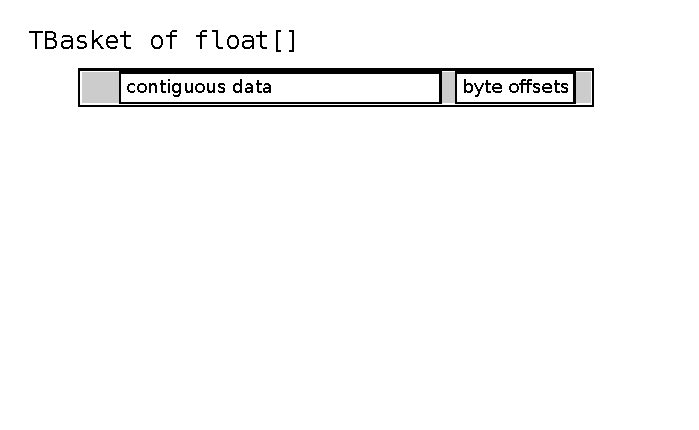
\includegraphics[width=\linewidth]{tbasket-to-awkward-1.pdf}}\only<2>{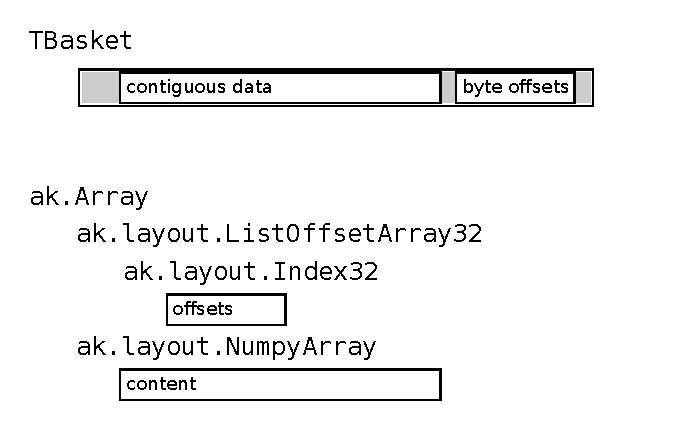
\includegraphics[width=\linewidth]{tbasket-to-awkward-2.pdf}}\only<3>{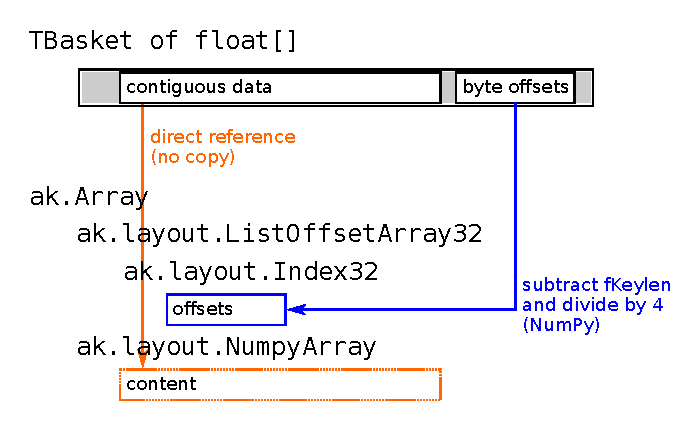
\includegraphics[width=\linewidth]{tbasket-to-awkward-3.pdf}}\only<4>{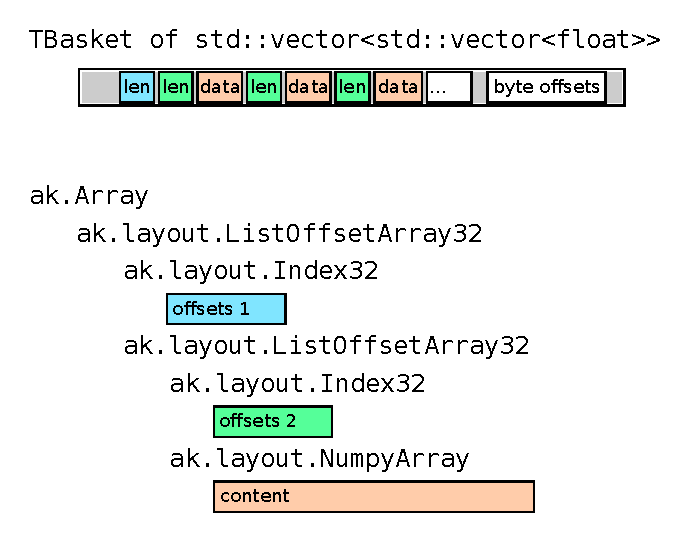
\includegraphics[width=\linewidth]{tbasket-to-awkward-nested.pdf}}

\column{0.3\linewidth}
\begin{onlyenv}<3>''Deserialization'' consists of $\mathcal{O}(1)$ metadata-only operations and $\mathcal{O}(n)$ vectorizable operations.
\end{onlyenv}\begin{onlyenv}<4>Record-oriented data, on the other hand, {\it must} be iterated sequentially, with control-flow decisions throughout.

\vspace{0.5 cm}
For Uproot, this means that reading lists of lists of numbers (in Python) is 460$\times$ slower than reading numbers (NumPy cast).
\end{onlyenv}
\end{columns}
\end{frame}

\begin{frame}{The general problem of deserialization}
\vspace{0.25 cm}
\Large
\begin{enumerate}
\item Data types are not known until you examine the data's schema.
\item Knowing data types is essential for generating fast code.
\end{enumerate}

\large
\vspace{0.25 cm}
\begin{columns}[t]
\column{0.001\linewidth}

\column{0.45\linewidth}
\uncover<2->{\textcolor{darkblue}{\underline{\bf Potential solutions}}}

\vspace{0.1 cm}
\uncover<2->{Generate deserialization code in a dynamic language, like Python.}

\vspace{0.1 cm}
\uncover<3->{Require a compilation step for every data file (like Protobuf).}

\vspace{0.1 cm}
\uncover<4->{JIT-compile the deserialization code (like ROOT, using Cling).}

\vspace{0.1 cm}
\uncover<5->{Use a parser combinator library.}

\vspace{\baselineskip}
\vspace{0.1 cm}
\uncover<6->{Create a lightweight/specialized virtual machine.}

\column{0.45\linewidth}
\uncover<2->{\textcolor{darkblue}{\underline{\bf Suitable for Uproot?}}}

\vspace{0.1 cm}
\uncover<2->{This is what Uproot does, and as we've seen, it's too slow.}

\vspace{0.1 cm}
\uncover<3->{That's a cumbersome workflow if you have several datasets.}

\vspace{0.1 cm}
\uncover<4->{Adding LLVM as a dependency would undermine portability.}

\vspace{0.1 cm}
\uncover<5->{ROOT deserialization requires advanced language features.}

\vspace{0.1 cm}
\uncover<6->{That's the subject of this talk.}
\end{columns}
\end{frame}

\begin{frame}{``Lightweight'' virtual machines?}
\vspace{0.25 cm}
\Large

The most numerous virtual machines are not Java, VirtualBox, Xen, etc., but regex string-matching.

\vspace{0.25 cm}
\begin{center}
\scriptsize
Ken Thompson, {\it Regular Expression Search Algorithm}, 1968.

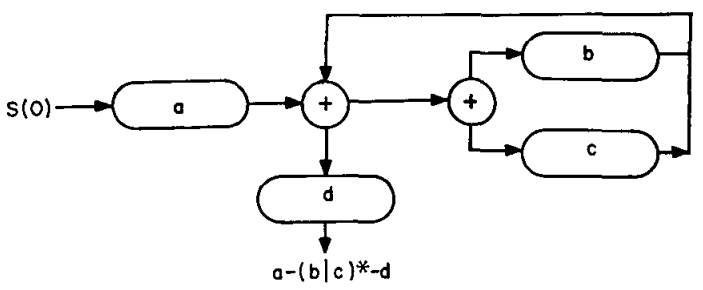
\includegraphics[width=0.5\linewidth]{thompson-regex-fig5.png}
\end{center}

\normalsize
\uncover<2->{A regex string like \mintinline{python}{"a(b|c)*d"} gets compiled into a finite state machine for fast execution. Limiting the scope of the machine provides opportunities for optimization.}

\vspace{0.25 cm}
\uncover<3->{Python's \mintinline{python}{struct} module (bytestring-parsing) and \mintinline{python}{numexpr} (math) are similar.}
\end{frame}

\begin{frame}{Another issue: Uproot and Awkward Array must be independent}
\large
\vspace{0.2 cm}
\begin{center}
\only<1>{
\includegraphics[width=0.85\linewidth]{awkward-uproot-interaction-1.pdf}}\only<2>{
\includegraphics[width=0.85\linewidth]{awkward-uproot-interaction-2.pdf}}\only<3->{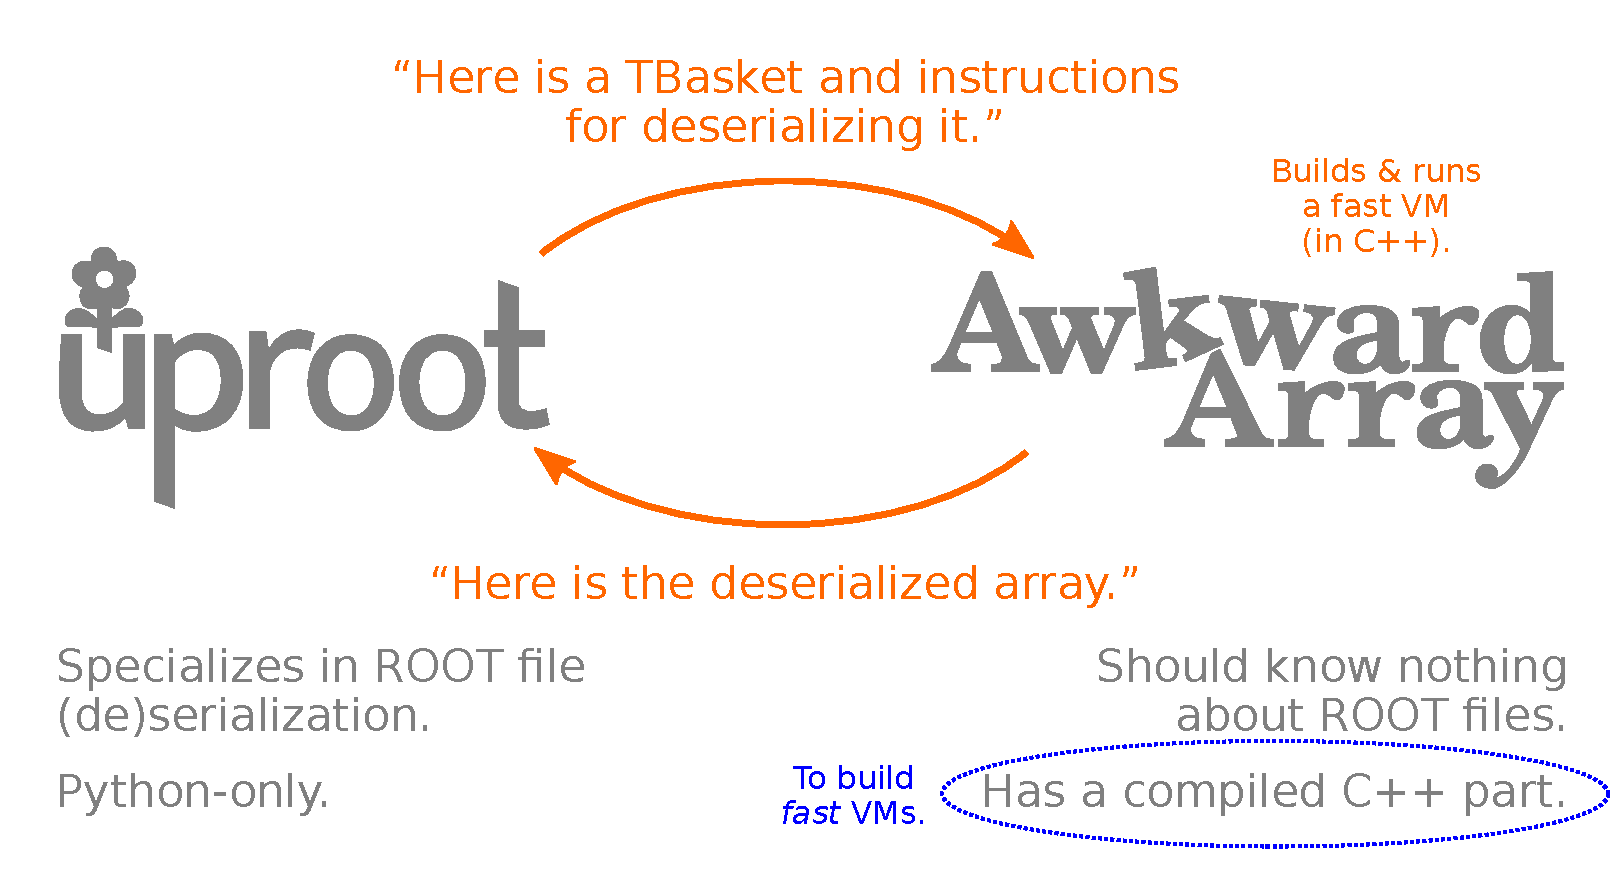
\includegraphics[width=0.85\linewidth]{awkward-uproot-interaction-3.pdf}}
\end{center}

\vspace{-0.15 cm}
\uncover<4->{\textcolor{darkblue}{Uproot needs a language to express how to deserialize a TBasket, but it doesn't need to be a human language.}}
\end{frame}

\begin{frame}{So, how about Forth?}
\vspace{0.28 cm}
\begin{columns}
\column{0.6\linewidth}
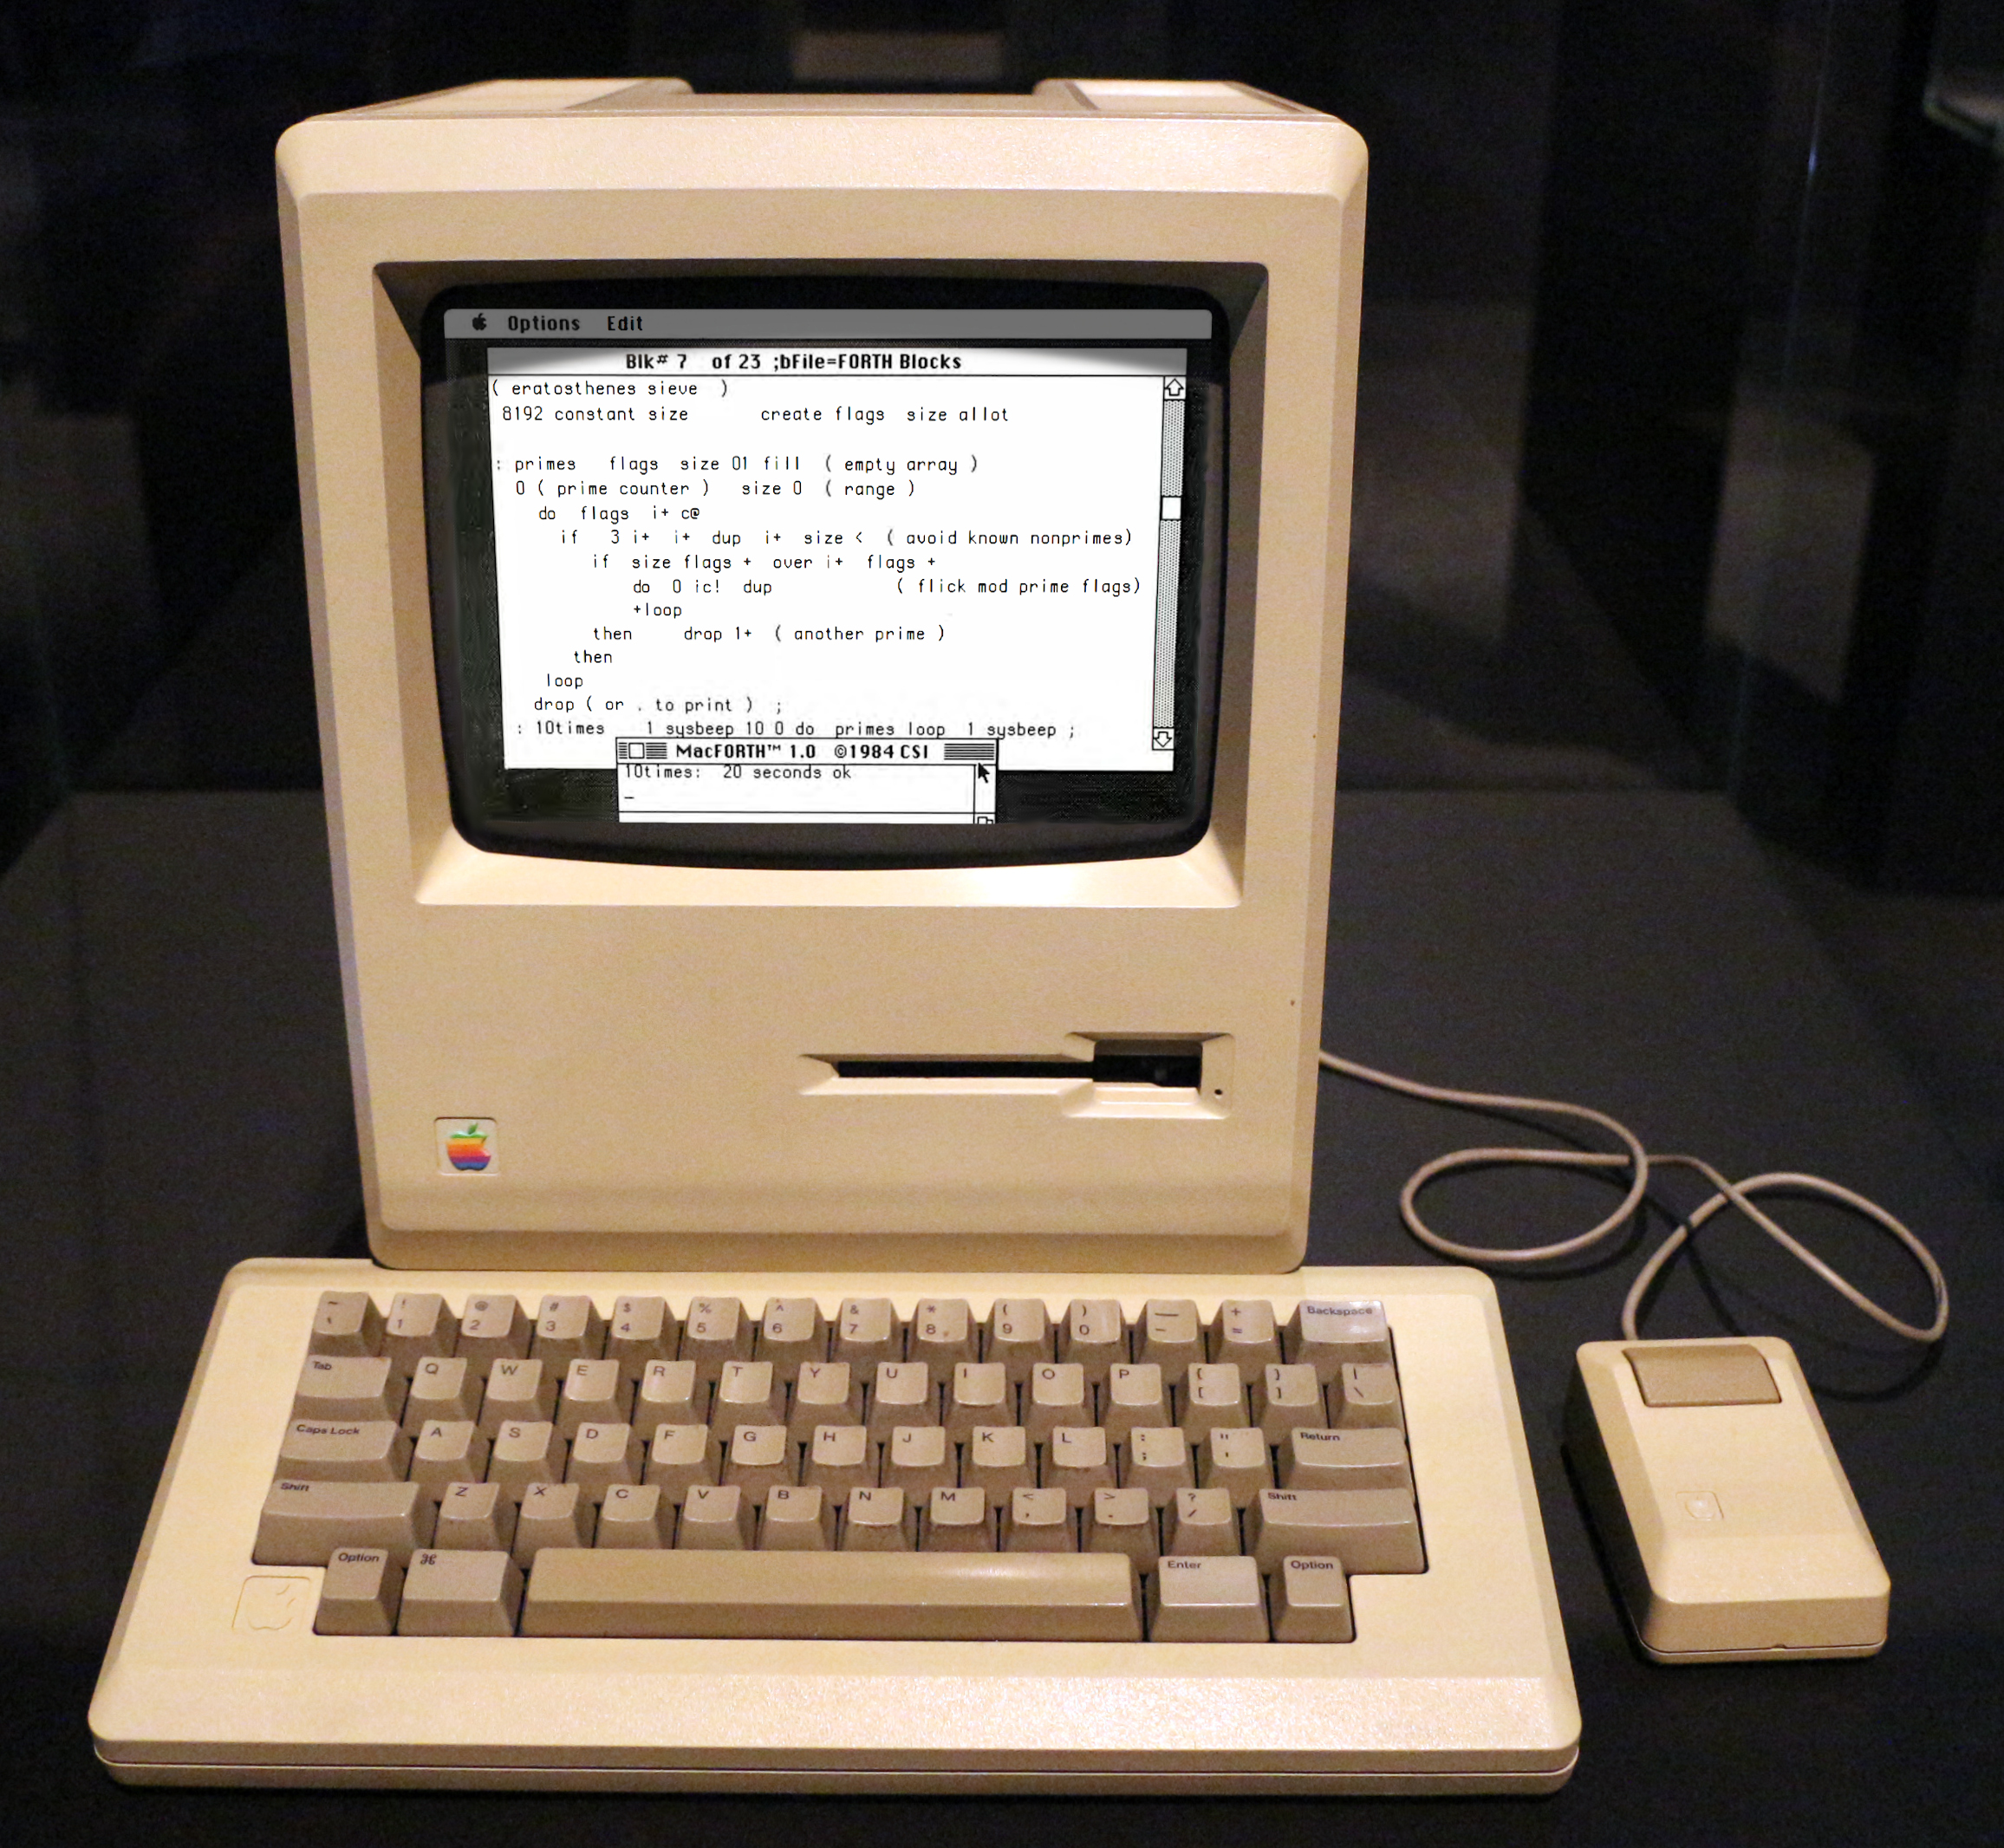
\includegraphics[width=\linewidth]{macintosh-forth-code.jpg}

\column{0.45\linewidth}
I heard about it through CollapseOS, which targets underpowered but ubiquitous hardware (Z80 chips).

\vspace{0.5 cm}
\begin{uncoverenv}<2->
Forth was invented in 1970 to control radio astronomy telescopes and was popular in early PCs because of the limited hardware.
\begin{itemize}
\item First Mac couldn't run a compiler; Forth was the only developer environment to make applications.
\end{itemize}
\end{uncoverenv}

\vspace{0.5 cm}
\uncover<3->{Almost no grammar, easy to generate. The Postscript language is a Forth.}
\end{columns}
\end{frame}

\begin{frame}{What does Forth look like?}
\large
\vspace{0.3 cm}
\mbox{ } \hfill 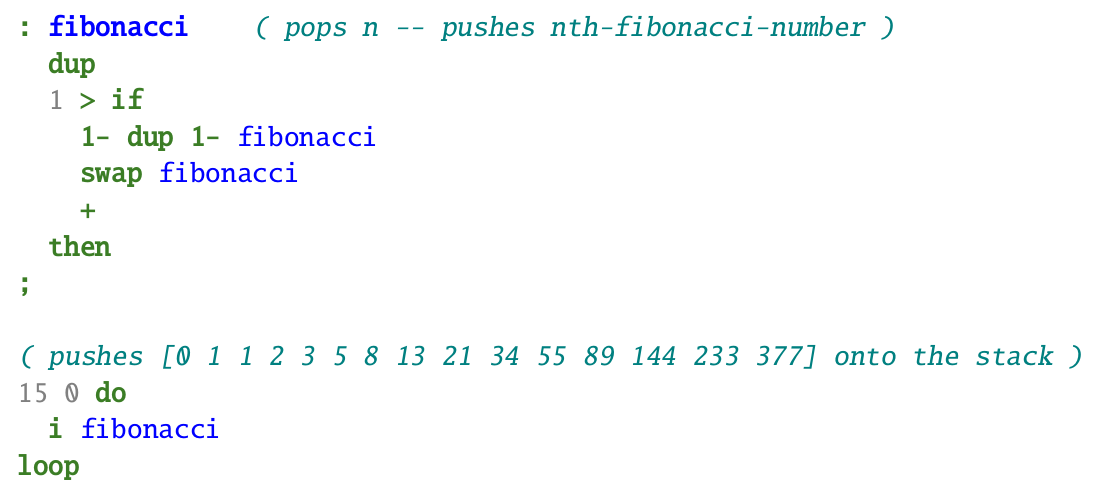
\includegraphics[width=0.93\linewidth]{forth-example.png} \hfill \mbox{ }

There's a global stack, words like ``\textcolor{gray}{\tt 1}'' push a number on the stack, and words like ``\textcolor{OliveGreen}{\tt\textbf{>}}'' and ``\textcolor{OliveGreen}{\tt\textbf{if}}'' pop values off the stack, apply operations, and push the result.

\vspace{0.2 cm}
Other than control flow like ``\textcolor{OliveGreen}{\tt\textbf{:}} \ldots\ \textcolor{OliveGreen}{\tt\textbf{;}}'' and ``\textcolor{OliveGreen}{\tt\textbf{do}} \ldots\ \textcolor{OliveGreen}{\tt\textbf{loop}},'' it goes left to right.
\end{frame}

\begin{frame}{AwkwardForth: a dialect of Forth with built-in parsing}
\large
\vspace{0.25 cm}
\begin{columns}
\column{1.05\linewidth}
Deserializing \mintinline{c++}{std::vector<std::vector<float>>} from a ROOT TBasket:
\end{columns}

\vspace{0.05 cm}
\mbox{ } \hfill 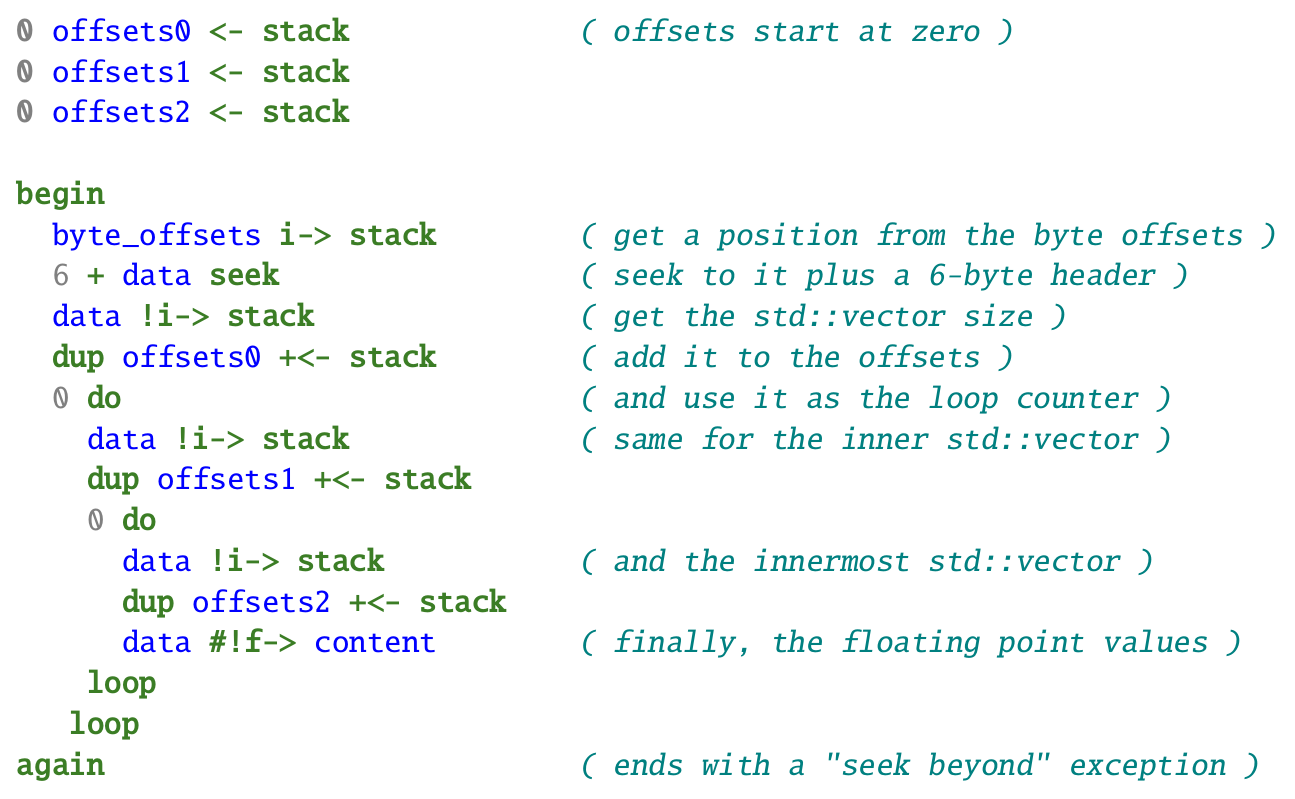
\includegraphics[width=0.83\linewidth]{forth-parsing-example.png} \hfill \mbox{ }
\end{frame}

\begin{frame}{Provides a way for Uproot to talk to Awkward Array}
\vspace{0.25 cm}
\begin{itemize}
\item Knowledge of ROOT I/O stays in Uproot.
\item Uproot generates an AwkwardForth program as a string (loose coupling).
\item Awkward Array builds and runs the machine to get an Awkward Array as output.
\item No humans need to read or write the Forth code (except for debugging).
\end{itemize}

\begin{columns}
\column{0.001\linewidth}

\column{0.55\linewidth}
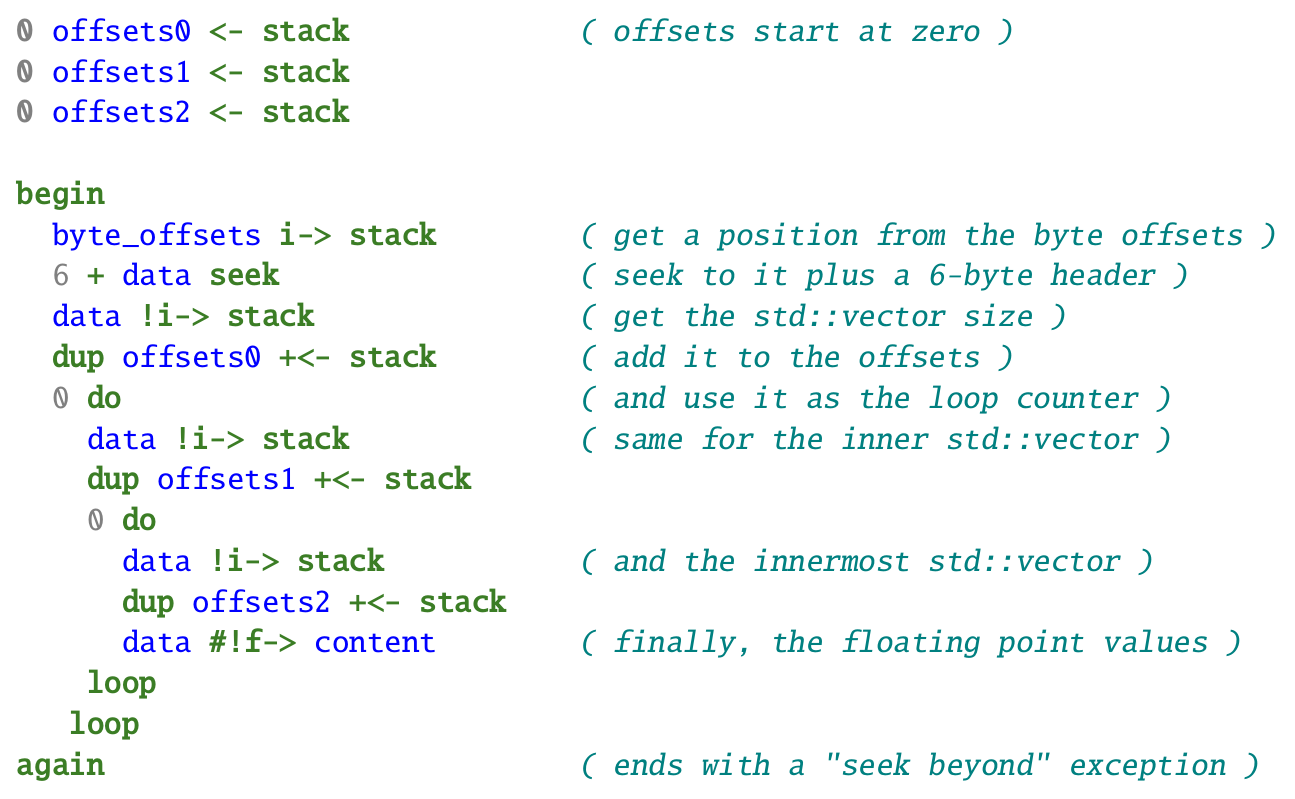
\includegraphics[width=1.1\linewidth]{forth-parsing-example.png}

\column{0.5\linewidth}
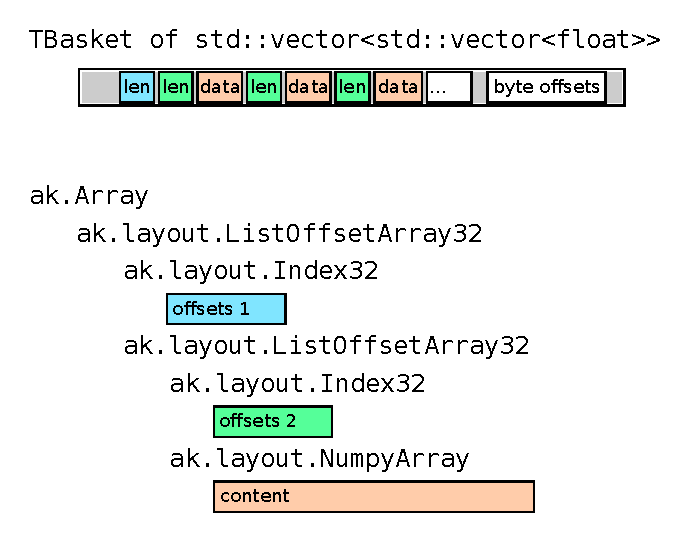
\includegraphics[width=\linewidth]{tbasket-to-awkward-nested.pdf}

\end{columns}
\end{frame}

\begin{frame}{Performance for ROOT deserialization (higher is better)}
\large
\vspace{0.2 cm}
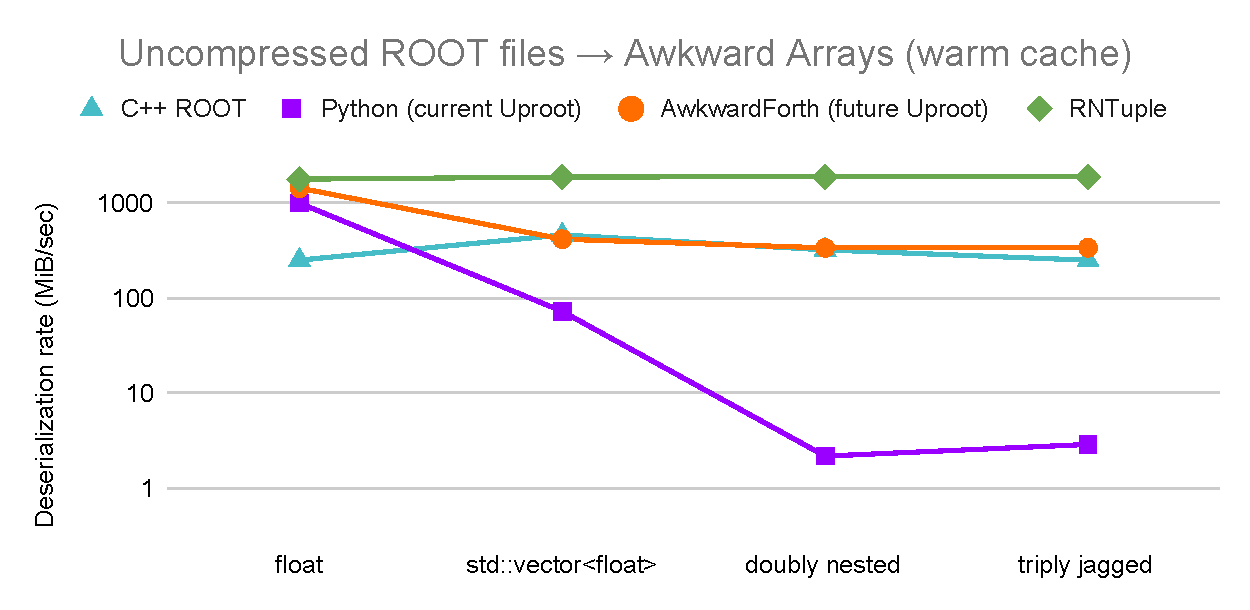
\includegraphics[width=0.95\linewidth]{AwkwardForth-performance-ROOT.pdf}

AwkwardForth is several times slower than compiled C++, but on par when data throughput is included. Compare also Python (current Uproot) and RNTuple.
\end{frame}

\begin{frame}{Performance for Avro deserialization (higher is better)}
\large
\vspace{0.2 cm}
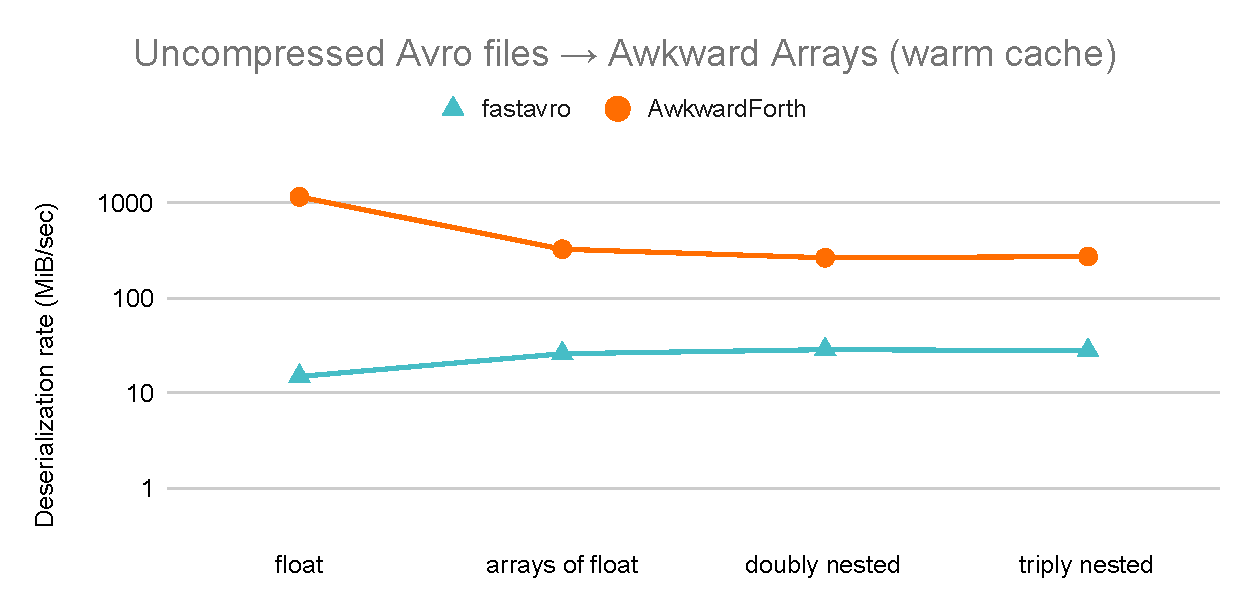
\includegraphics[width=0.95\linewidth]{AwkwardForth-performance-Avro.pdf}

Since the language can handle any parsing problem, consider other formats like Avro. The \mintinline{python}{fastavro} library is C code, but doesn't know data types in advance.
\end{frame}

\begin{frame}{Performance for Parquet deserialization (higher is better)}
\large
\vspace{0.2 cm}
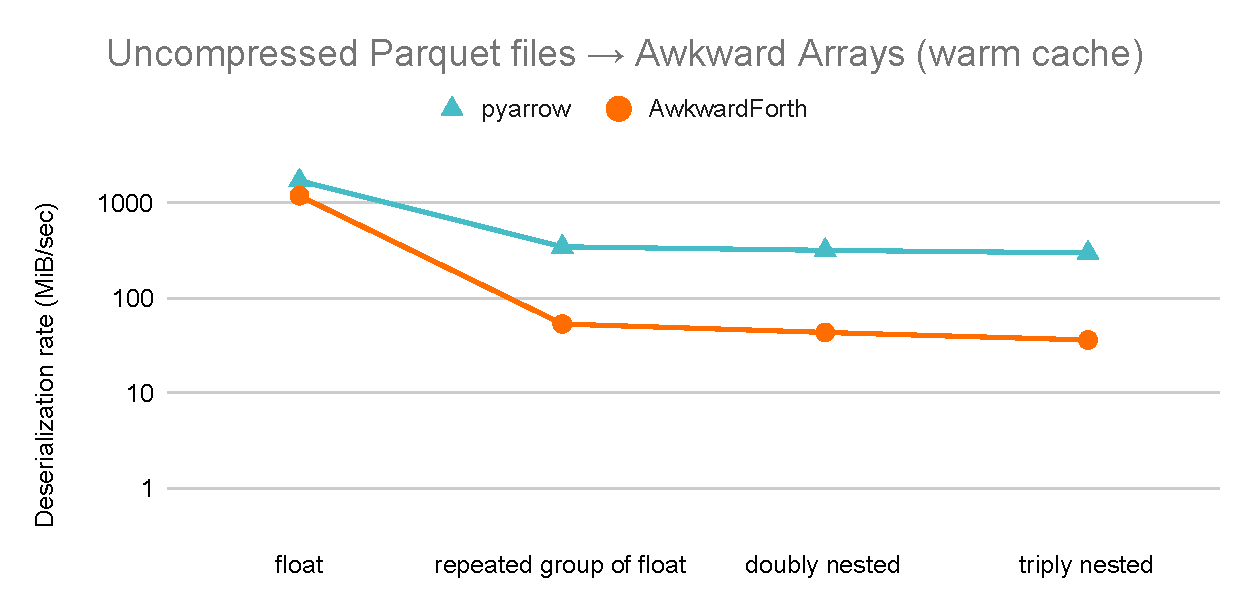
\includegraphics[width=0.95\linewidth]{AwkwardForth-performance-Parquet.pdf}

Keep going: consider Parquet. Here, AwkwardForth doesn't do as well as \mintinline{c++}{pyarrow}'s C++ parser because Parquet is a columnar format (like RNTuple).
\end{frame}

\begin{frame}{Parallel processing performance of AwkwardForth and Python}
\large
\vspace{0.2 cm}
\begin{columns}
\column{0.5\linewidth}
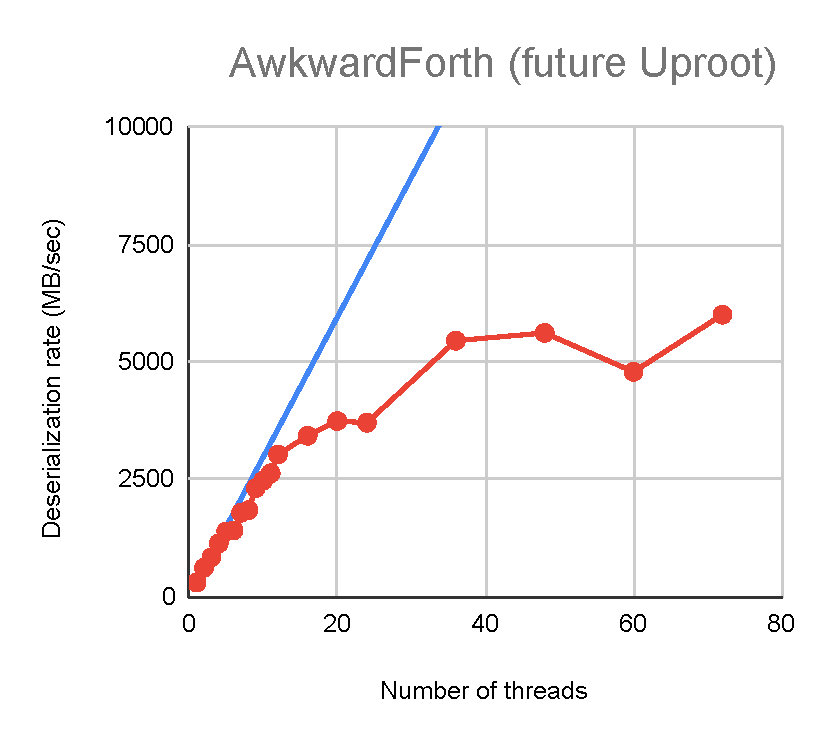
\includegraphics[width=\linewidth]{AwkwardForth-scaling.pdf}

\column{0.5\linewidth}
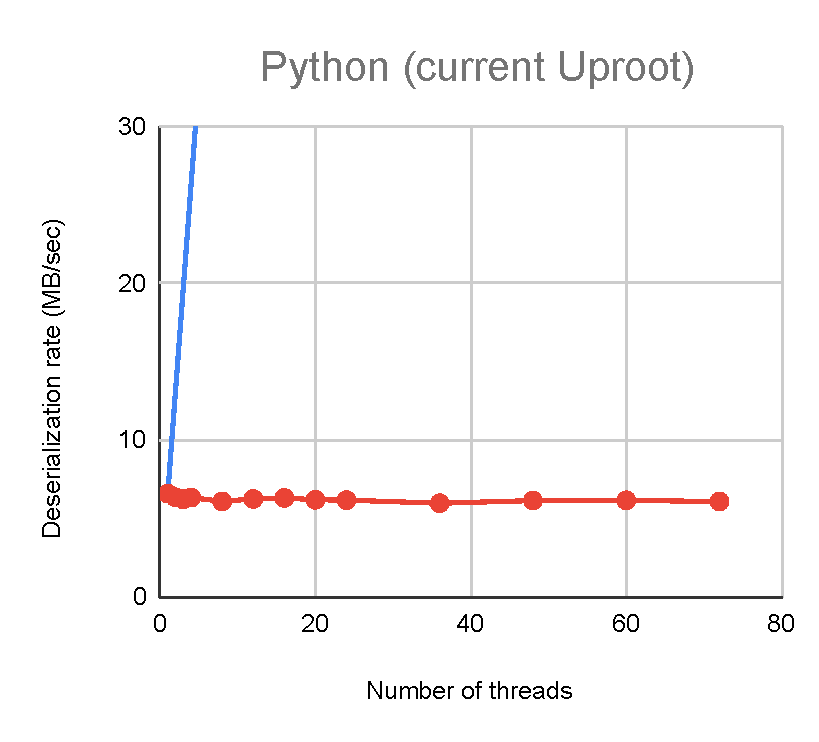
\includegraphics[width=\linewidth]{Python-scaling.pdf}
\end{columns}

AwkwardForth machines are lightweight: we can make one per thread. Python is inhibited by the GIL. Scales linearly up to RAM access ceiling (5 GB/sec).
\end{frame}

\begin{frame}{Closing remarks}
\Large
\vspace{0.25 cm}
\setbeamercolor{alerted text}{fg=darkblue}
\begin{itemize}[<+-|alert@+>]\setlength{\itemsep}{0.2 cm}
\item See the paper for more details, including application to \mintinline{python}{TypedArrayBuilder}.
\item A complete Forth implementation is small ($<$ 5k lines of C++) and fast (5~ns per instruction).
\item Particularly useful for communicating algorithms between software libraries with restricted (sandboxed) runtimes.
\item Uproot's Python-generating routines must now be supplemented by Forth-generating routines; targeting the end of this year.
\item You might want to consider a similar technique in your project. \scriptsize

\vspace{0.1 cm}
\hfill\href{https://github.com/scikit-hep/awkward-1.0/tree/1.2.3/src/libawkward/forth}{\textcolor{blue}{\underline{https://github.com/scikit-hep/awkward-1.0/tree/1.2.3/src/libawkward/forth}}}

\end{itemize}
\end{frame}

\end{document}
